\subsection{Controllers for z$_{\mathrm{I}}$ Direction}
As in the case of the controller in the $x_{\mathrm{I}}$ and $y_{\mathrm{I}}$ directions, a cascade approach is chosen fo the$z_{\mathrm{I}}$ direction.

The transfer function to control the velocity is obtained, where the four motor velocities as input and the velocity in the z-direction in the inertial system, as output. From \autoref{eq:FinalLinearEquationZ}, with the corresponding translational linearized block diagram in \autoref{fig:TranslationalLinearModelBlockDiagram}, the linear transfer function for the z-direction is readily obtained.
%
\begin{flalign}
  \frac{\dot{z}_I}{\omega_{\mathrm{sum}}} &= \frac{ \frac{1}{4}\ (-2 k_{\mathrm{th}})\ \overline{\omega}_{sum} }{ m s }  \label{eq:linearTransferFunctionZ}
\end{flalign}

\begin{where}
  \va{\dot{z}_I}{is the velocity in the z-direction in the inertial system}{}
  \va{\omega_{\mathrm{sum}}}{is the sum of velocities to be controlled}{}
  \va{\overline{\omega}_{\mathrm{sum}}}{is the sum of rotor velocities in equilibrium}{}
\end{where}

This system has a pole in zero and a negative gain, which means that the locus on increasing gain will drive the system into the right half plane and make it unstable. As in the case of the other controllers, an integral term is added to reduce the effect of input disturbances.
 
The root locus of the system, which now contains two poles in zero, will branch along the imaginary axis. To avoid oscillations the two loci are attracted by the use of a zero, placed on the left real axis as seen in \autoref{fig:rootLocusOfZwithPI}.

\begin{figure}[H]
	\centering
	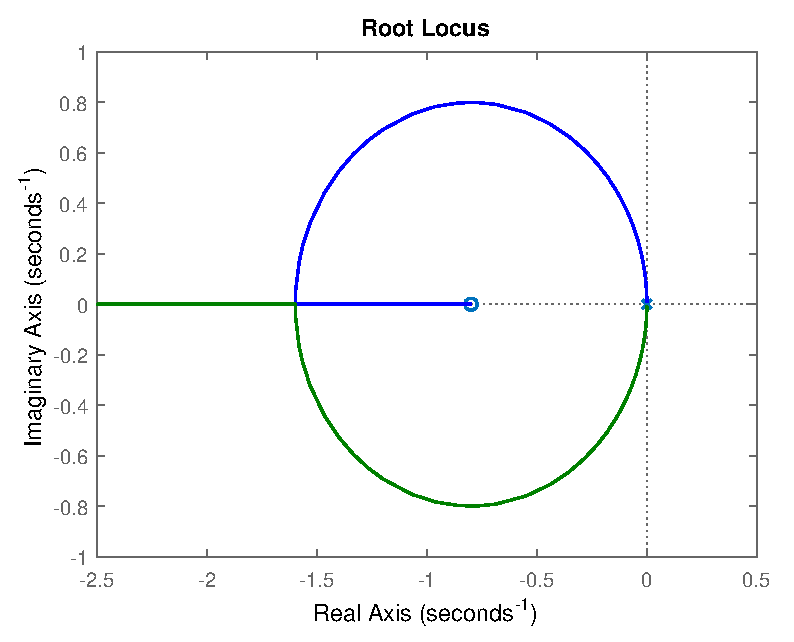
\includegraphics[width=.6\textwidth]{figures/rootLocusOfZwithPI.pdf}
	\caption{Root locus of the system with PI control. The zero is placed in (0,-0.8).}
	\label{fig:rootLocusOfZwithPI}
\end{figure}

The zero is placed and the gain is scaled to achieve a good rise time with a reasonable control action while keeping the zero far enough from the poles, such that the integrator is not canceled. The zero is placed in -0.8 on the real axis and with a gain of -201.

The final expression for the velocity controller is
%
\begin{flalign}
    C_{\dot{x}_I}(s)&= -280 \frac{s+0.8}{s} \label{eq:Czdot}
\end{flalign}
%

The position controllers for $z_{\mathrm{I}}$ directions can be designed using the same procedure as for $x_{\mathrm{I}}$ and $y_{\mathrm{I}}$. As in the previous case, the position transfer function is an integrator.
%
\begin{flalign}
    G_{z_I}(s)&=\frac{z_I (s)}{\dot{z}_I (s)}=\frac{1}{s}  \label{eq:Gz}
\end{flalign}

The proportional gain is chosen so that the bandwidth of the position loop is 3 times lower than that of the velocity loop, that can be seen in the close loop bode of the velocity control loop.
%
\begin{figure}[H]
    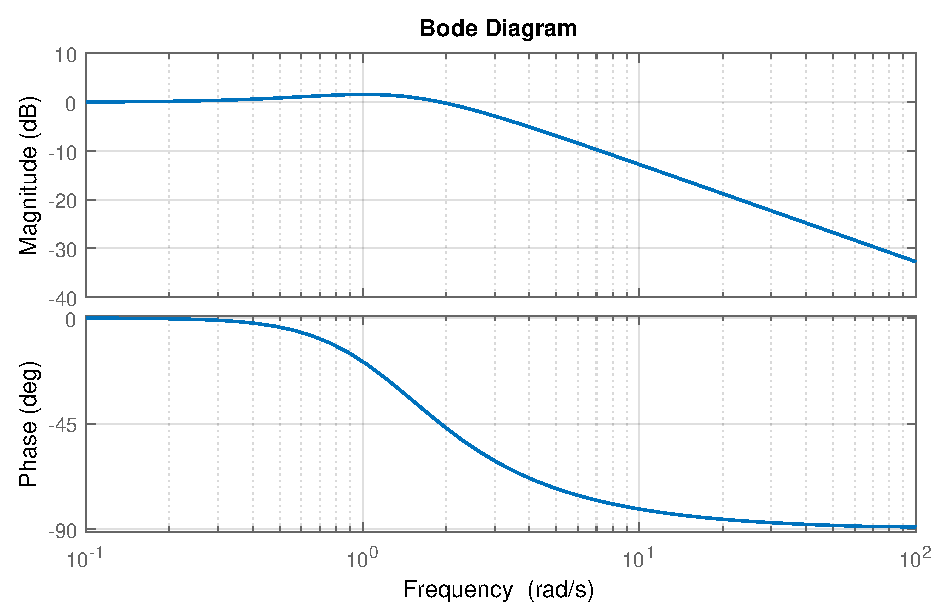
\includegraphics[scale=.7]{figures/bodeVelocityZ}
    \centering			
    \captionof{figure}{Closed loop bode of the plant and the controller for the $z_{\mathrm{I}}$ translational velocity.} 
    \label{fig:bodeVelocityZ}
\end{figure}
%
This defines it to be 1 rad $^-1$. Since the pant has already this bandwidth, the gain is just 1 in this case.
%
\begin{flalign}
    C_{z_I}(s)&= 1\label{eq:Cz}
\end{flalign}
%


















% The step response of the linear system with the PI controller is seen on \autoref{fig:stepOfZwithPI}.
%
%\begin{figure}[H]
%	\centering
%	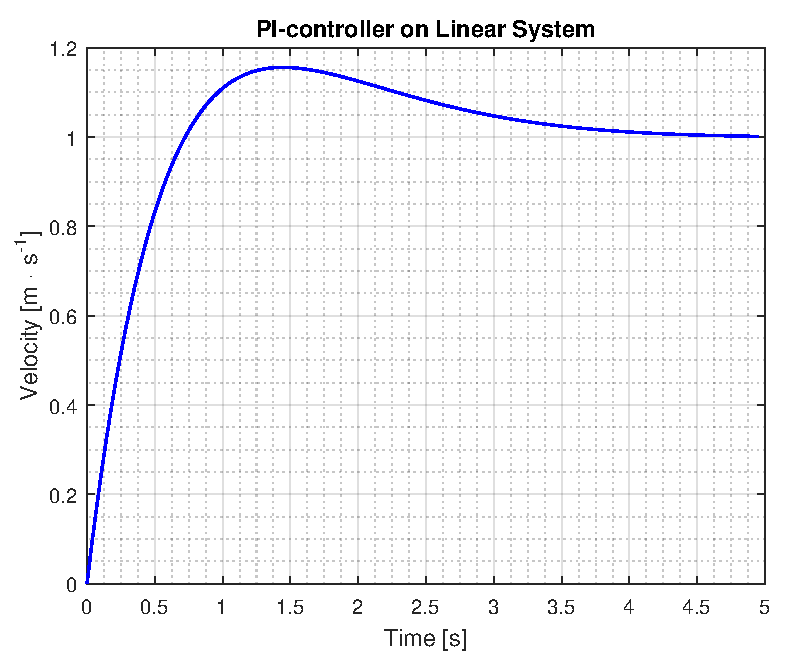
\includegraphics[width=.6\textwidth]{figures/stepOfZwithPI.pdf}
%	\caption{Step response of the linear system with PI control.}
%	\label{fig:stepOfZwithPI}
%\end{figure}
%


%
%If a gain of $-200$ is applied, the controller will bring the velocity to \SI{1}{m \cdot s^{-1}} in approximately \SI{2}{s}, see \autoref{fig:ZstepPcontrolLinear}.
%
%\begin{figure}[H]
%    \centering
%    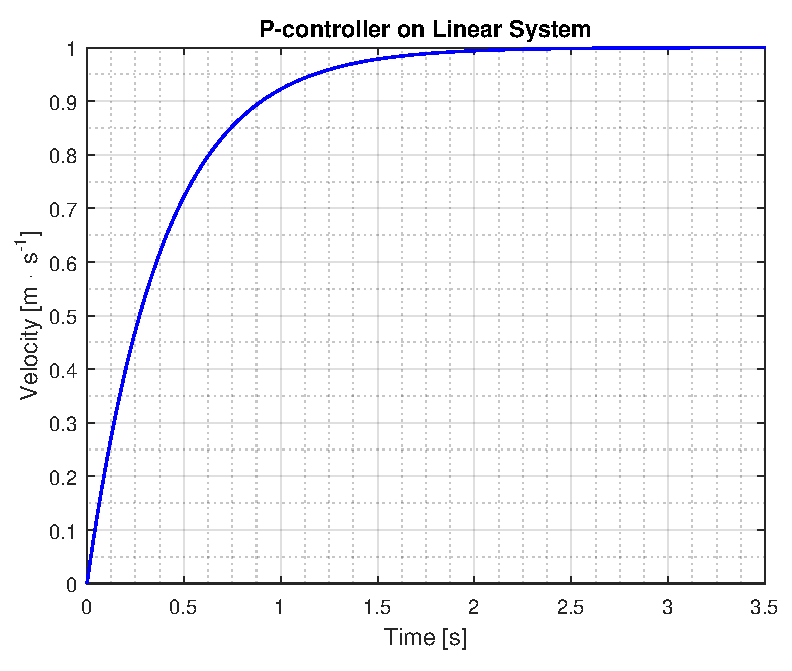
\includegraphics[width=.6\textwidth]{figures/ZstepPcontrolLinear.pdf}
%    \caption{Step response of the linear transfer function with a P-controller with a gain of $-200$.}
%    \label{fig:ZstepPcontrolLinear}
%\end{figure}
%
%%However a P-controller does not account for input disturbances, and neither does the integrator in the plant. Therefore, if the equilibrium speed of the rotors has an offset under some flight conditions, this error will not be accounted for.
%To see this effect, the P-controller is tested on the nonlinear model with an added difference of \SI{5}{rad \cdot s^{-1}} in each of the four needed equilibrium speeds in the model. The simulation is seen below in \autoref{fig:ZstepPcontrolNonlinear}, where the reference input is subjected to a step of \SI{1}{m \cdot s^{-1}}, however, the velocity stabilizes instead at \SI{0.9}{m \cdot s^{-1}}, revealing a steady state error.
%
%\begin{figure}[H]
%    \centering
%    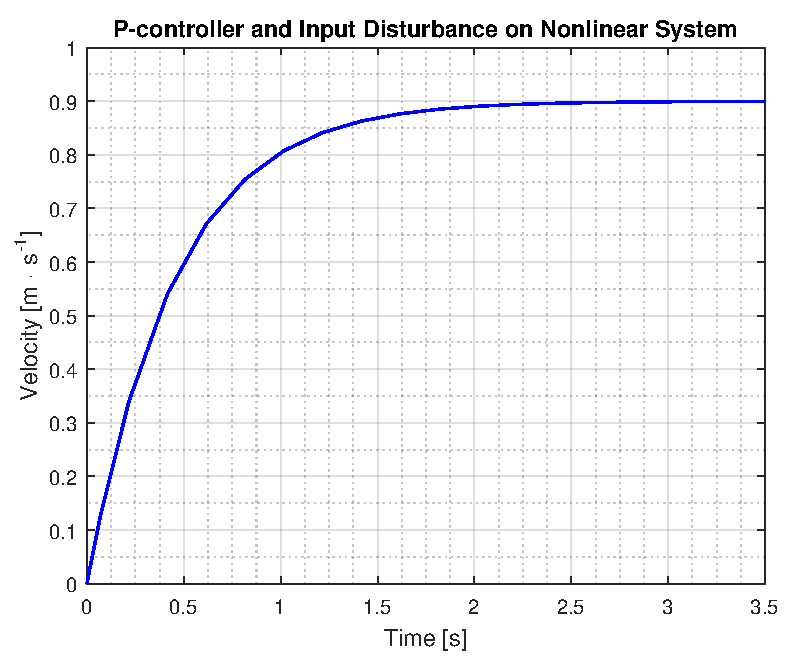
\includegraphics[width=.6\textwidth]{figures/ZstepPcontrolNonlinear.pdf}
%    \caption{Step response of the nonlinear transfer function with a P-controller with a gain of $-200$.}
%    \label{fig:ZstepPcontrolNonlinear}
%\end{figure}
%%
%%In order to remove the steady state error an integrator is introduced to the controller. 
%
%
%
